\documentclass[a4paper,11pt]{article}
\setlength{\topmargin}{-.5in}
\setlength{\textheight}{9in}
\setlength{\oddsidemargin}{.125in}
\setlength{\textwidth}{6.25in}
\usepackage[pdftex]{graphicx}
\makeatletter
\renewcommand\paragraph{%
   \@startsection{paragraph}{4}{0mm}%
      {-\baselineskip}%
      {.5\baselineskip}%
      {\normalfont\normalsize\bfseries}}
\makeatother

\begin{document}

% The Title page
\begin{titlepage}
\begin{center}
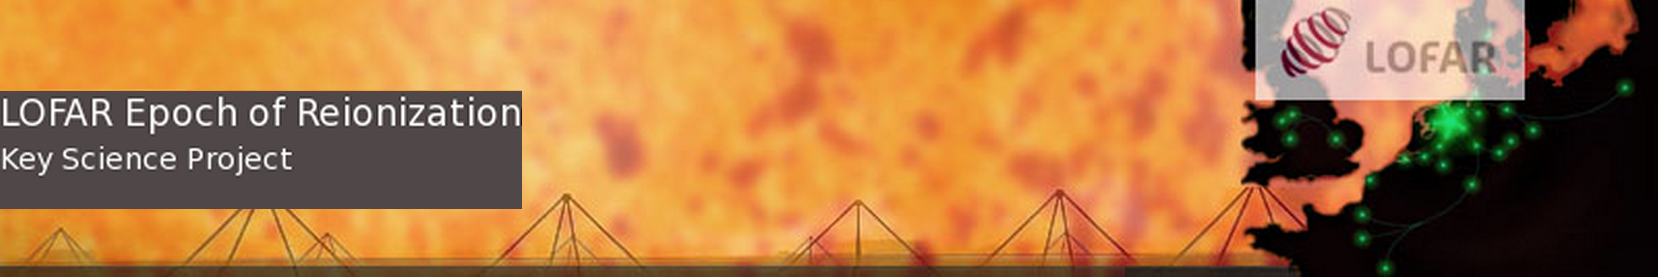
\includegraphics[width=0.8\textwidth]{fig/eorlogo}\\[3cm]    
\textsc{\LARGE LEDAMA Software Package}\\[0.5cm]
\vfill
{\large
\emph{Oscar Martinez} \\
University of Groningen \\
Kapteyn Astronomical Institute \\
Groningen \\
The Netherlands \\
\today}
\end{center}
\end{titlepage}


% INDEX
\tableofcontents
\newpage

\section{Introduction}

Here we describe the software package LEDAMA (\textbf{L}OFAR \textbf{E}oR \textbf{DA}ta \textbf{MA}nagement). The main concept of this package is that it is based on \textit{LModules}. A \textit{LModule} is basically a script performing some tasks. See section \ref{sec:lmodules} for a detailed description of the \textit{LModules}. LEDAMA contains all the code required for the:

\begin{itemize}
    \item LOFAR EoR data management, processing and analysis. LEDAMA aims to provide tools (\textit{LModules}) for the processing of a large number of measurement sets. These \textit{LModules} need, as input, \textit{RefFiles}. A \textit{RefFile} is a file which contains the locations of measurement sets.
      
    \item LEDDB handling (for more information regarding the database see the LEDDB document), i.e. how to fill and browse the database. This also includes the tools for the diagnostic data visualization and the LEDDB web user interface (UI). The \textit{LModules} for the diagnostic data visualization need, as input, \textit{DiagFiles}. A \textit{DiagFile} is a file with the references to diagnostic data stored in the LEDDB.
      
    \item Cluster monitoring. This is based on daemons running in each node of the LOFAR EoR cluster that are collecting network traffic, CPU, GPU (currently disabled), memory and disk usage information. There is a tool within the LEDDB web for the displaying of the collected data. There is also a \textit{LModule} that can be used for that purpose.
\end{itemize}

\section{Package overview}

The root directory of the LEDAMA package contains the following sub-packages:

\begin{itemize}
    \item \textit{datamanagement} contains all the required code to perform data management (also processing) tasks.
    \item \textit{dataanalysis} contains tools for diagnostic data visualization and for extraction of statistical information of the data in a measurement set.
    \item \textit{doc} contains all documentation related to LEDAMA, LEDDB and the LOFAR EoR data management and processing.
    \item \textit{leddb} contains the code to handle the LEDDB.
    \item \textit{web} contains the code for the LEDDB web UI (including the web server and the client-side JavaScript/JQuery code).
    \item \textit{nodes} contains the code for the cluster monitoring.
    \item \textit{extscripts} contains scripts that do not use \textit{LModules}. They are independent and self-contained scripts that do not use any other LEDAMA code.
\end{itemize}

In the root directory the following files can also be found:

\begin{itemize}
    \item \textit{config.py}: The LEDAMA configuration file. More information on section \ref{sec:config}.
    \item \textit{daemon.py}: Contains a generic daemon class which is the parent class of the node monitoring daemon.
    \item \textit{DiagnosticFile.py}: Contains a class to handle (read and write) \textit{DiagFiles}.
    \item \textit{diagoperations.py}: File with methods to get the diagnostic data (\textit{getGain}, \textit{getQTS}, \textit{getQFS} and \textit{getQBS}). It also contains methods to define/handle the diagnostic tables partitions.
    \item \textit{MovieInfoFile.py}: Contains a class to handle the Gain movies that are added in the LEDDB.
    \item \textit{msoperations.py}: Important file that contains methods to extract information (project, epoch, field \ldots) from a Measurement Set. It also contains the method to extract the large bulk of data (i.e. the \textit{DATA} column)
    \item \textit{MSP.py}: Contains a class to handle the measurement sets that are added in the LEDDB.
    \item \textit{nodeoperations.py}: File with some methods to get measurement sets locations from nodes.
    \item \textit{PrettyTable.py}: Contains a class to get an ASCII table nicely formatted.
    \item \textit{ReferenceFile.py}: Contains a class to handle (read, write and combine) \textit{RefFiles}.
    \item \textit{tasksdistributor.py}: Important file that contains code to distribute different tasks. This is used, by the \textit{LModules}, to do simultaneous processing in different cores and/or nodes.
    \item \textit{utils.py}: File that contains useful methods used all over the LEDAMA package.
\end{itemize}
 
There are the files \textit{ExecuteLModule}, \textit{LModule.py}, \textit{LModuleLoader.py} and \textit{LModuleOptions} but they are fully described in section \ref{sec:lmodules}.

\section{Software repository, installation and configuration}
\label{sec:config}

The LEDAMA code can be downloaded from:.

\begin{verbatim}
git clone https://github.com/oscarmartinezrubi/ledama
\end{verbatim}

The LEDAMA package has some requirements (python modules) to meet in addition to the LOFAR pipeline software (NDPPP, BBS, sagecal, etc.):

\begin{itemize}
	\item numpy
	\item matplotlib
	\item pyrap (tables and images)
	\item parmdb
	\item ppgplot
	\item tk (Tkinter)
	\item psycopg2
	\item cherrypy
	\item generateDS.py (http://www.rexx.com/~dkuhlman/generateDS.html).	
\end{itemize}

After all the requirements are fulfilled you just need to download the LEDAMA code to some location and add this location to the \textit{PYTHONPATH}.

LEDAMA is configured through the \textit{config.py} file in the root directory of the package (there is also a specific configuration file for the web server but this will be discussed in the web section, i.e. \ref{sec:webconfig}).

The main parameters that need to be configured in the \textit{config.py} file are:

\begin{itemize}
    \item \textit{LEDAMA\_ABS\_PATH}: The path to the directory where the LEDAMA is installed. 
    \item \textit{INIT\_FILE}: The initialization file that will be sourced (before anything else) in all the remote tasks of the \textit{LModules}.
    \item \textit{LEDDB\_NAME} and \textit{LEDDB\_HOST}: The name and host where the LEDDB is running.
    \item \textit{FULL\_ACCESS\_USERS}: Only some users can make serious modifications in the database, handle the nodes daemons and use the GRID NL code. Some \textit{LModules} check the user before running the code. Currently, \textit{lofardata} is the only user which such privileges (and it is the one in charge of the LEDDB filling and maintenance). If you would like to change this, remember that you also need to set the proper permissions in the LEDDB database.
    \item \textit{LEDDB\_BACKUP\_HOST} and \textit{LEDDB\_BACKUP\_FOLDER}: The host and folder where the backup of the LEDDB is executed and stored (by \textit{lofardata} user). There is a cron task that needs to be set up in order to perform the backup, see section \ref{sec:leddbcron}.
    \item \textit{LEDDB\_WEB\_DIR}: The web folder directory. This is the location from where the web server is executed.
    \item \textit{WEB\_USERS}: To run the LEDDB web server there should be a special user different than the full access user (\textit{lofardata}), currently it is the user \textit{leddbweb}. If you would like to change this, remember that you also need to set the proper permissions in the LEDDB database (we advise to use a user with read-only access).
    \item \textit{NODE\_MONITOR\_FOLDER}, \textit{NODE\_MONITOR\_TYPE}, \textit{NODE\_MONITOR\_DB\_NAME} and \textit{NODE\_MONITOR\_DB\_HOST}: The Cluster Monitor (or Node Monitor) requires a folder where to store the several daemons information. It has two modes: using a DB or using files. If you decide to use a DB you must define the host and name (Note that this DB can be the same than LEDDB but it is not recommended).
\end{itemize}

\section{\textit{LModules}}
\label{sec:lmodules}

The core of LEDAMA are the LModules. All the tasks that can be done with LEDAMA are done trough the \textit{LModules}. There is a interface class in the root directory of LEDAMA named \textit{LModule.py}.
Each sub-package of LEDAMA contains several implementations of \textit{LModule}.

Within the \textit{LModule} there is a standard way of specifying the arguments that a certain implementation can have. This is done via the class in \textit{LModuleOptions.py}.

There is a common command-line launcher for all the \textit{LModules} named \textit{ExecuteLModule}. Few comments on this:

\begin{itemize}
    \item Type \textit{ExecuteLModule -h} to see all the possible \textit{LModules}.
    \item To run a certain \textit{LModule} you must type: \textit{ExecuteLModule [LModule name]}.
    \item For more information about any \textit{LModule} type \textit{ExecuteLModule [LModule name] -h}.
\end{itemize}

Few generic comments on the \textit{LModules}:

\begin{itemize}
    \item In some \textit{LModules} options multiple values can be specified. In such case separate them with commas. In the case of integers (also for the names of the nodes) you can define ranges with $..$ or $-$. For example \textit{1..3}, \textit{1-3} and \textit{1,2,3} is all the same. You can also use double $..$ to specify a step different than $1$. For example \textit{0..6..2} is the same than \textit{0,2,4,6}.
    \item In almost all the \textit{LModules} there are two distribution options (in addition to other options in each particular case). With these options you can define how the several tasks of the \textit{LModule} will be distributed/executed in the nodes of the LOFAR EoR cluster:
    \begin{itemize}
        \item Number of simultaneous nodes running tasks: This option is important for example in tasks that require NFS traffic.
        \item Number of simultaneous processes per node: With this option you can limit how many simultaneous tasks are done in each node. This option is important for not overloading the nodes.
    \end{itemize}  
    \item In almost all the \textit{LModules} you can also define a initialization file (the default one is specified in LEDAMA configuration). This file will be sourced before each remote task execution. This is used to give you control over which software/version/build is used.
    \item In some \textit{LModules} you can define a logs folder where all the processes running the remote tasks will write their progress.
    \item In many \textit{LModules} you can use the option \textit{query} that will show the commands instead of executing them.
\end{itemize}

\textit{ExecuteLModule} uses \textit{LModuleLoader.py} to load the \textit{LModules}.

In sections \ref{sec:datamp}, \ref{sec:dataanal}, \ref{sec:leddb}, \ref{sec:web} and \ref{sec:nodes} we describe the several sub-packages of the LEDAMA package. In each one we describe its \textit{LModules}.

\section{Cron tasks}

In the data management (\ref{sec:datamp}), the leddb (\ref{sec:leddb}) and the nodes (\ref{sec:nodes}) sub-packages there are a set of scripts that are meant to be run as cron tasks. In each sub-package we will describe them.

\section{Frequent scripts}

In the data management (\ref{sec:datamp}), data analysis (\ref{sec:dataanal}) and the leddb (\ref{sec:leddb}) sub-packages there are a set of scripts that are meant to ease the execution of very frequents tasks. In each sub-package we will describe them.  

\section{Data management and processing (\textit{datamanagement} sub-package)}
\label{sec:datamp}

This sub-package contains the code to ease the LOFAR EoR data management and processing. It contains modules, cron scripts, frequent scripts and the code to handle the SIPs.

\subsection{\textit{LModules}}

If you want to use LEDAMA (and its \textit{LModules}) for data management and processing tasks, in general you need a \textit{RefFile}. This file will contain the list of measurement sets that you want to manage/process.

In the \textit{LModules} where the input is a \textit{RefFile} (almost all of them) the same action is done to all the measurements sets of that \textit{RefFile} and, via the distribution options, you can decide the number of simultaneous measurement sets being processed in each node and the number of simultaneous working nodes.

So, the most important \textit{LModules} are the ones that create \textit{RefFiles} (do not worry there are many of them and also from the LEDDB). These ones and the rest of \textit{LModules} are described below.

\subsubsection{Data management}

In this section we present all the \textit{LModules} related to data management.

\paragraph{CreateRefFileFromPath}

Creates a \textit{RefFile} by specifying paths and/or nodes (without using the LEDDB).
You can decide if only packed data is considered (i.e. TAR or BVF files).
In addition you can also specify to only check the locations (paths/nodes).
In this way the measurement sets are not read (this can be specially useful if you think that the measurement sets may be locked, i.e. being used)

\paragraph{CreateRefFileFromRefFile}

Creates a \textit{RefFile} from other \textit{RefFiles} specifying excluded or included patterns, SB indexes and nodes.

\paragraph{CreateRefFileFromTarget}

The main archive in the LOFAR EoR project is in the Target LTA facilities (See \textit{Handling the LOFAR EoR data} document). This \textit{LModule} create a \textit{RefFile} from data in the archive.
You have to specify the target area: TARGET\_E\_EOR is where the processed data is archived and TARGET\_F\_EOR is where the raw data is temporally stored.
You also need to specify the relative directory. In this case the directory is always directly the LDS name, for example L123456 or L123456\_001 if it is the 15ch version. Remember that each different version must have a version index. Currently there is an agreement to use ``\_001'' for the 15 channels version, ``\_002'' for the 3 channels version and ``\_003'' for the 1 channel version.

\paragraph{CopyData}

This is a very important \textit{LModule} since it is the one used to copy the data to/from the EoR cluster from/to the LTA archive (mainly Target).

It copies the data in a \textit{RefFile} to the locations (paths and nodes) specified by the user. You can specify to copy certain SB indexes. It also has a \textit{resume} option, if it is activated the copy will not be executed if the data is already copied (this can only be checked if the data is being copied to the EoR cluster)

In this case you can specify a status path where the progress of the copies are logged. We can use this folder in the \textit{CheckData} to get a overview of the copy status.

\paragraph{CheckData}

Checks the availability of data pointed by \textit{RefFile} by comparing the observed size with the one in the RefFile. The status path of a copy in progress can also be used. In this case the speed and the remaining time of the copying process is also computed.

\paragraph{DeleteData}

Deletes data pointed by a \textit{RefFile}. You can also delete the parent path in each node.

\paragraph{ExecuteCommandOnData}

Executes a command in all the measurement sets pointed by the \textit{RefFile}. Before execution it is recommended to use query option. The command is defined by using keyword that will be replaced in each MS. You can choose to use SSH or NFS.

\paragraph{ChmodData}

Changes the permissions (\textit{chmod}) to the data pointed by \textit{RefFile}.

\paragraph{CleanEmptyLDSPaths}

Deletes empty LDSs paths. All the transfers and archiving processes generate many folders that after a while become empty. This \textit{LModule} can be used to clean them.

\paragraph{CompareData}

Compares the contents of some \textit{RefFiles}. It checks them using the SB index and the size.
If only one \textit{RefFile} is given it only checks that the provided SBs are in the \textit{RefFile} and that they are not multiple.
If multiple \textit{RefFiles} are given the first one is used as reference for the sizes and then it checks that the SBs in the first \textit{RefFile} are also present in the second one and that they have the same size.

\paragraph{ExtendPermissionsOnData}

Extends writing permissions to all the MS in the \textit{RefFile} to the user (it also changes the parent path). This is useful when you want to give permissions to only one user.

\paragraph{MD5SumData}

Creates a md5sum of the data pointed by a \textit{RefFile}.

\paragraph{MSInfo}

Shows information about the contents of a \textit{RefFile} or of a single MS. If a \textit{RefFile} is provided it assumes that all the measurement sets have same averaging properties.

\paragraph{PackData}

Packs (TAR) the data in a \textit{RefFile}.

\paragraph{UnPackData}

Unpacks (TAR) the data in a \textit{RefFile}.

\paragraph{ShowProcesses}

Shows all the processes owned by the user which command name (as specified by \textit{ps -aux}) contains all the words specified by the user. It can also be used to kill them (but it is always recommended to run it first without the kill option just to be sure of what would be killed).

\subsubsection{Data processing (pipeline)}

In this section we present all the \textit{LModules} related to the LOFAR EoR data processing (pipeline jobs), i.e. how to average the data, flag it, obtain quality information, calibrate it, make images, etc.

As explained in the \textit{Handling the LOFAR EoR data} document there are some standard processing steps:

\begin{itemize}
    \item From the raw data (64 channels, 2 seconds) we create the first NDPPP averaged version (15 channels, 2 seconds). Before averaging we flag the data.
    \item From the first version (15 channels, 2 seconds) we create the second NDPPP version (3 channels, 2 seconds).
    \item From the second version (3 channels, 2 seconds) we create the third NDPPP version (1 channels, 10 seconds).   
    \item The second and third versions are calibrated with SAGECal and/or BBS.
\end{itemize}

All the processing can be done simultaneously to all the measurement sets of an observation (few hundreds) thanks to the \textit{LModules} presented in this section.

In all these \textit{LModules} the standard distribution options, logs path, query and initialization file options are available.

\paragraph{CreateNDPPPParsetFiles}

The execution of the NDPPP \textit{LModule} requires to create, first of all the NDPPP parset files. This \textit{LModule} is meant to do this and it requires a output folder where the new parsets will be stored and a NDPPP template parset file where the lines related to the measurement set will be replaced in each case.

You also need to specify the path where the new measurements sets will be stored (if there are new measurements sets to be created). The nodes that will be used are defined in the \textit{LaunchNDPPP} \textit{LModule}.

\paragraph{LaunchNDPPP}

After creating the NDPPP parset files you are ready to launch all the NDPPP executions. Use this module for this purpose. You need to specify the folder where the several parset files are located. By default the nodes that contains the original data are used and hence the new creates files will be in the same node than the original ones (the path was decided in the \textit{CreateNDPPPParsetFiles}). However, you can define a different set of nodes, in which case NFS will be used to access the data.

\paragraph{LaunchAOFlagger}

This \textit{LModule} is used to run the \textit{aoflagger} to all the measurement sets of a \textit{RefFile}. The \textit{aoflager} can also be run within the NDPPP and this is actually what we normally do in the LOFAR EoR processing.

\paragraph{UnFlagData}

At any time you can unflag all the measurement sets pointed by a \textit{RefFile} with this module.

\paragraph{LaunchAOQuality}

This \textit{LModule} is used to collect quality statistics (using \textit{aoquality}) of the measurement sets. This will create the quality tables within each one of the measurement sets. The \textit{aoquality} can also be run in NDPPP (in fact, it is the default behavior when creating new files). In the LOFAR EoR processing we normally run \textit{aoquality} through NDPPP.

\paragraph{LaunchCalibrateSA}

This module is used to calibrate the data using the stand-alone BBS. It does not require VDS or GDS files, only a \textit{RefFile}, and it is the current used way of running BBS in the LOFAR EoR processing.

You need to define a parset file describing the several calibration steps that you wish to do and a sky model file. You can specify a execution path where BBS will run in each remote host and this is recommended because some ancillary files are created for each calibration process.

\paragraph{CreateVDSFiles}

The execution of \textit{LaunchBBS} \textit{LModule} (which is not currently being used in the LOFAR EoR processing) requires to create the GDS and VDS files. This \textit{LModule} is used to create the VDS files. It will create one VDS file for each measurement set in the specified \textit{RefFile}.

\paragraph{CreateGDSFiles}

This \textit{LModule} is used to create the GDS files required by the \textit{LaunchBBS} \textit{LModule}. You can define which SBs goes in each GDS file. There are a set of predefined GDS schema that you can choose with some keywords.

\paragraph{LaunchBBS}

After creating the several VDS and GDS files you are ready to run BBS. In this \textit{LModule} you need to specify a parset file and a sky model file (as in the calibrate-stand-alone). In this case you also need to provide the DB details.

\paragraph{CleanData}

Cleans (removes) the indicated column in the measurement sets pointed by the provided \textit{RefFile}

\paragraph{ReadCorrXY}

In previous releases of SAGECal it was required to create a BVF file from a measurement set before being able to calibrate the data. This is not the case any more.

This obsolete \textit{LModule} creates BVF files from the measurement sets pointed by a \textit{RefFile}.

\paragraph{WriteCorrXY}

As in the previous case, this module is obsolete. It updates the column of the measurement sets pointed by the \textit{RefFile} with the calibrated data from the related BVF file.

\paragraph{LaunchSagecal}

Calibrates the measurement sets in a \textit{RefFile} with the SAGECal. It requires a cluster file and a sky model file as well as the output folder where the calibration solutions will be stored.

\paragraph{CreateCASAImagerParsetFiles}

The execution of the \textit{casa} imager \textit{LModule} requires, first of all, to create its parset files. This \textit{LModule} creates them by providing a template file and the output folder for the parset files. You also need to specify a extension that will be added in the generated image files names.

\paragraph{LaunchCASAImager}

Launches the \textit{casa} imager processes in all the measurement sets of a \textit{RefFile}.

\paragraph{CreateAWImagerParsetFiles}  

The execution of the \textit{awimager} \textit{LModule} requires, first of all, to create its parset files. This \textit{LModule} creates them by providing a template file and the output folder for the parset files. You also need to specify a extension that will be added in the generated image files names.

\paragraph{LaunchAWImager}

Launches the \textit{awimager} processes in all the measurement sets of a \textit{RefFile}.

\paragraph{CreateMWImagerParsetFiles}

This deprecated \textit{LModule} was used to create the parset files required for the \textit{mwimager} which is no longer installed in the LOFAR EoR cluster.

\paragraph{LaunchMWImager}

Launches the deprecated \textit{mwimager} processes in all the measurement sets of a \textit{RefFile}.

\paragraph{AddImagingColumns}

Adds imaging columns to the measurement sets pointed by a \textit{RefFile}.

\paragraph{MakeBeam}

Make the beam tables in each one of the measurement sets pointed by a \textit{RefFile}.
This code only works in node079 because this is the only node where the related software is installed.

\paragraph{RescaleFitsImage}

Re-scale a FITS image.

\paragraph{SetMount}

Set \textit{MOUNT} to $ALT-AZ$ in all the ANTENNA tables of all the measurement sets pointed by a \textit{RefFile}.

\subsubsection{Archive}

Here we present the \textit{LModules} related to data archiving. As already stated, the main archive used for LOFAR EoR data is Target (which is part of the LOFAR LTA). Currently the connection to Target is done using FDT (http://monalisa.cern.ch/FDT/) so there are few modules related to it.

We also use (but in a much lower scale) the archiving facilities provided by SARA as part of the GRID NL infrastructure (part of the LOFAR LTA uses it). There are two \textit{LModules} related to it.

Finally, the last two \textit{LModules} are for creating and getting SIPs. The SIPs are XML files that contain meta-data of the measurement sets (actually of any file/folder to archive in the LOFAR LTA)

\paragraph{FDTDaemonsManager}

Manages (starts and stops) FDT servers in several nodes of the LOFAR EoR cluster. This is only meant for testing purposes.

\paragraph{GetFDTFileList}

Writes a file with the content of the specified directory in the store. It can also be used (if none directory is not specified) to show the possible directories.

The \textit{CreateRefFileFromTarget} module uses the code defined in this \textit{LModule}.
        
\paragraph{TestFDT}

Starts client processes in some nodes of the LOFAR EoR cluster that try to connect to a remote host and port. It requires a log path where the progress of each FDT process is stored.

This module is used to test FDT connections with Target.

If you run this module you will need to stop with \textit{Ctrl-C}. It is recommended that afterwards you use \textit{ShowProcesses} \textit{LModule} to kill any remote FDT process that may still be hanging in the nodes of the LOFAR EoR cluster.   

\paragraph{GetTestFDTSpeed}

When running \textit{TestFDT} you can use this other \textit{LModule} to get the total speed of the connection.

\paragraph{GRIDBringOnline}

Bring online files in GRID. Most probably this does not work and you need to ask it explicitly to Target LTA people (Hanno Holties or Adriaan Renting)

\paragraph{InitGRID}

In order to be able to copy data from GRID NL infrastructure you first need to initialize the GRID software in the specified LOFAR EoR nodes. Otherwise, the copy data module will not work.

Currently this is not working since there are some issues with the certificates.

\paragraph{GetSIPs}

Get the SIPs from one of these 2 options (in both options you have to manually specify the project):
\begin{itemize}
  \item From copy-paste table download from MOM (or a single DataProduct Id).
  \item From an observation Id from the LTA catalog.
\end{itemize}

In principle, the LTA people should provide in short term a tool to get all the DataProduct Ids from an observation name / id which will ease getting SIPs since right now it is tedious to copy-paste the data from MOM for each observation.

\paragraph{CreateSIPs}

Create SIPs for all the measurements sets pointed by the \textit{RefFile}.
We assume all the measurements sets are of the same version (or LDSBP, see LEDDB document for information). For the new SIPs the LDSBP information is used (and the LDSBPUpFile if specified).
For each measurements set its new SIP is a direct update from the input SIP (and they are related trough the SB index)

\subsection{Cron tasks}

There is only one cron task in the \textit{datamanagement} sub-package. It is the  \textit{CronCleanEmptyLDSPaths.py} and it is used to clean once per month the unused directories in the EoR cluster.

As in the rest of cron tasks, they must be properly set in the related node using the tool crontab. See the file to know in which node and when the task should run.

\subsection{Frequent tasks}

Whenever there is a new observation the procedure is as follows: 

\begin{itemize}
	\item We get the raw data from Target to EoR data. 
	\item Some (usually 3: 15, 3 and 1 channels) averaged versions are created and processed.
	\item We archive the averaged/processed versions
\end{itemize}

Hence, there are some scripts to do these frequent tasks:

\begin{itemize}
	\item The \textit{gencopytarget2eor.py} generates the commands to copy a new observation from Target to EoR cluster (obviously using \textit{CopyData} \textit{LModule}). It only requires the \textit{RefFiles} with the data in Target, the names of these \textit{RefFiles} must have the following format: LXXXXX[\_VVV][\_BY]\_TARGET.ref where [VVV] is optional and is for the version (if not specified it assumes version 0) and BY is also optional and is for the beam (for example B0 for beam 0 or B1-6 for beams 1 to 6). You also need to specify the nodes that will be used. 
	\item The \textit{genpreproc.py} generates the commands to create the average versions. It assumes that all the data is in the standard LOFAR EoR cluster locations, i.e. \\ /dataX/users/lofareor/[pipeline]/LXXXXX\_VVV. You need to provide which disks are used for each version in addition to the nodes where the raw data is located (and where the other versions will be created).
	\item The \textit{gencopyeor2target.py} generates the commands to archive the several averaged versions. It requires the LDS name and the \textit{RefFiles} pointing to the data.  
\end{itemize} 

\subsection{SIPs}

As previously stated the SIP files are XML files required by the LOFAR LTA catalog. They are required (or will be soon enough) when archiving the data in the LTA. In this sub-package there are the files required to handle SIPs. The XSD definition, a SIP python API generated with an external library called generateDS.py (http://www.rexx.com/$\sim$dkuhlman/generateDS.html) and the SIPIOHandler which is the class used to read/write SIPs.

\section{Data analysis (\textit{dataanalysis} sub-package)}
\label{sec:dataanal}

This sub-package contains the code to do some data analysis, mainly in the form of some \textit{LModules} for diagnostic data visualization but also a very useful \textit{LModule} to get statistics of the measurement set data.

In order to visualize diagnostic data the first needed thing is a \textit{DiagFile}. In the next section we present the \textit{LModules} that use \textit{DiagFiles} to do their job. But here we also want to give an example of usage of a \textit{DiagFile} out of the \textit{LModules}.

\subsection{Example of usage of a \textit{DiagFile}}

You can use the python interface class \textit{DiagnosticFile} in the file \textit{ledama.DiagnosticFile}  in the LEDAMA root directory to load the diagnostic data and use it the way you want. For example:
\begin{verbatim}
        >>> from ledama.DiagnosticFile import DiagnosticFile
        >>> diagFile = DiagnosticFile(diagFilePath)
        >>> data = diagFile.queryData()
        >>> print len(diagFile.data)
\end{verbatim}
In the example we open a \textit{DiagFile}, we query the data (this is actually querying the data from the LEDDB so it can take a while) and then we show the number of rows. In this case we are querying the default header, even though we could query a different header. See the \textit{QueryTables.py} file in \textit{leddb/query} sub-package to see the different available columns. 

\subsection{\textit{LModules}}

Here we detail the several available \textit{LModules} for data analysis. 

\subsubsection*{Diagnostic plotters}

There is a class called \textit{DiagnosticLoader} that deals with loading any type of diagnostic data from the LEDDB. There is also an abstract plotter that contains all the code to plot the diagnostic data.

Then, there are four of specific plotters, one for each diagnostic type: \textit{GainPlotter, QBSPlotter, QFSPlotter and QTSPlotter}. The main features of these plotters are:

\begin{itemize}
\item Data is queried from LEDDB every time you plot.
\item There is a re-usage of already generated axis.
\item Select which polarizations to plot and which complex coordinates to use.
\item Choose the X axis you want to plot: TIME\_UTC\_NORMAL, TIME\_UTC\_WRAP\_BLANK, TIME\_UTC\_DAILY, TIME\_HOUR\_ANGLE and FREQ\_NORMAL
\item With sub-plot and color keys you can define how the data will be plotted. You can specify for which parameters you will have a new sub-plot and for which ones a new color in each sub-plot. The options for the keys are: l (LOFAR\_DATASET), f (CENTRAL\_FREQUENCY), s (STATION), p (POLARIZATION), r (DIRECTION\_RA), d (DIRECTION\_DEC), q (QUALITY\_KIND) and b (STATION\_2). Multiple parameters keys are also valid.
\item Define the X axis resolution (use this to speed up very large data analysis) and also the Y axis range.
\end{itemize}

\subsubsection*{GainAnimationSingleStation}

Makes an animation of gain solutions for a single station. The x axis of the plots is frequency and the animation is in time.

\subsubsection*{GainAnimation}

Very complex \textit{LModule} to generate Gain solutions movies of all stations and some measurement sets. See the document \textit{Description and usage of gainanim.py} for more information on this tool.
In fact there are two versions of this tool, the one presented here gets the data from the LEDDB and there is another one (in sub-package \textit{extscripts}) that loads the gain solutions directly from the files and not the LEDDB. 

\subsubsection*{UsedStations}

Plots a representation of the used stations during the observations.

\subsubsection*{ASCIIStats}

Writes in an ASCII file statistics of the data (not the diagnostic data). The input can be a measurement set path, a \textit{RefFile} or a GDS file. 
The statistics to compute and which data (column, times, channels, etc.) to use are specified as options.

\subsection{Frequent tasks}

There is a script for generating the commands to create movies from LDSBP IDs. From time to time, we have to run this script to generate the movies from the latest added gain solutions.

The suggested procedure is to get the list of LDSBPs that have GAIN solutions but still do not have movies. We select all these LDSBP and use this script to generate the commands to get the movies.

It is recommended to run this script in node007 where all the movies are stored and use as output path /data3/users/lofareor/movies/. This script is not cron because it is very consuming and it can be run in any node (since the data is queried from the LEDDB). So, the suggestion is to manually run this script once per month and use all the nodes in the EoR cluster thar are free at that time.

\section{LEDDB (\textit{leddb} sub-package)}
\label{sec:leddb}

This sub-package contains all the code to handle the LEDDB. For more information on the database see the \textit{LEDDB document}.

In addition to cron tasks, frequent scripts and \textit{LModules} there is another folder named \textit{query} that contains the query engine that is used when browsing the database (mainly using the LEDDB web). All these folders are described in the following sections.

There are also a set of files in this sub-package:

\begin{itemize}
	\item \textit{Connector.py}: We use the python module \textit{psycopg2} to interface with the LEDDB PostgreSQL database. The class \textit{Connector} is used to establish a connection with the database.
	\item \textit{LEDDB\_ER.erm} is not a python module, it contains the Entity-Relationship (ER) diagram of the LEDDB. In order to open this file you need the Eclipse plug-in ERMaster (http://ermaster.sourceforge.net).
	\item \textit{Naming.py} is a module that contains all the string constants used to refer to the LEDDB tables and columns.
	\item \textit{LEDDBOps.py} is a module that contains very important methods used to interact with the database, i.e. update, insert, select and delete operations.
	\item \textit{MSPUpdater.py} contains a class to add the information related to a measurement set (through an instance of \textit{MSP} python class) in the LEDDB.
	\item \textit{DiagnosticUpdater.py} contains a class to add diagnostic information related to a measurement set in the LEDDB. It uses the \textit{diagoperations.py} methods to access the diagnostic data.
	\item \textit{LDSBPUpFile.py} contains a class used to manually update a LDSBP and its description of the processing steps of the data (This is required for the SIPs generation).
\end{itemize}

\subsection{\textit{LModules}}

In this section we describe the \textit{LModules} for the LEDDB.

\subsubsection*{CreateLEDDB}

This module creates all the tables and functions of the LEDDB. Before executing this module you must have created the database using \textit{createdb} command.

\subsubsection*{DeleteLEDDB}

This module delete all the tables and functions related to the LEDDB. After executing this module you also need to execute \textit{dropdb} command to complete remove all the LEDDB.

\subsubsection*{BackupLEDDB}

This \textit{LModule} backup each individual table of the LEDDB in a selected directory. It implements a smart backup strategy based in the fact that the old diagnostic partitions (which contain the largest amount of data) do not change quite often, so there is no need to regenerate a backup of a partition if it has not changed compared to the last backup.

\subsubsection*{RestoreLEDDB}

This \textit{LModule} restore a LEDDB from a backup directory. As in \textit{CreateLEDDB} it requires to run the \textit{createdb} command before attempting to restore the database.

\subsubsection*{SizeLEDDB}

Gives the size of the database and of each one of its tables.

\subsubsection*{CreateLEDDBPartitions}

It creates the diagnostic partitions. The partitions that need to be created depend on the partitioning key, in our case the measurement set identifier. So, the more measurement set in the database the more partitions we need. This module must be run often in order to generate the partitions before we actually need them.

\subsubsection*{CreateRefFileFromLEDDB}

Creates a \textit{RefFile} from data in the LEDDB. It uses the API provided by the query engine (see section \ref{sec:query}).

\subsubsection*{CheckLDSBPs}

It compares for an observation (or many) two different LDSBPs given by the provided arguments.

\subsubsection*{CheckUnrefMSPs}

Localizes in the EoR cluster measurement sets that are not in the LEDDB.

\subsubsection*{CreateLDSBPUpFile}

Creates a \textit{LDSBPUpFile} from \textit{HISTORY} tables of the measurement sets and the current information in the LEDDB. Regarding the HISTORY tables, it assumes that all the measurement sets of the LDSBP have the same HISTORY table.

The created file needs to be modified describing the processing steps that have been done to the data. Afterwards you can use \textit{UpdateLDBSP} to commit the update the LEDDB content with the new information. 

This information will be only used in the SIPs generation.

\subsubsection{Add}

There are many modules to add data in the LEDDB depending on where the data is. For the data in the EoR cluster we normally use the \textit{UpdateLEDDBNode} module. In this case the data is accessible and we can extract all the information from the measurement sets. This section contains the modules that deal with adding measurement sets in the LEDDB that are not accessible (not in the EoR cluster) and hence we can not get much information from them.
In such case there is a common strategy, if there is the same measurement set (same LDS, version and SB index) in the EoR cluster (or it has existed) we can get the information from its entry in the LEDDB.

\paragraph*{AddRefFile}

Add all the measurement sets pointed by the \textit{RefFile} in the LEDDB. This can be used for data in and out of the EoR cluster.

\paragraph*{AddEmptyLDSBP}

Add a LDSBP and the MSs related to the measurement sets from an ASCII file extracted MOM. This is only used to add frequency information of the SBs of a LDS/version. Note that none MSP is added.

\paragraph*{AddFDTFileList}

Add references to LEDDB from a \textit{FDTFileList}. This is a file obtained with a line per \textit{GetFDTFileList} \textit{LModule} with a measurement set with 2 fields, the first field is the size and the second one is the relative path. This \textit{LModule} is deprecated since you can directly create \textit{RefFiles} from Target and use \textit{AddRefFile}.

\paragraph*{AddCatFileList}

Add references to LEDDB from a CatFileList. This file has a line per measurement set with 4 fields, the second field must be the path and the third the size. We also need a host:port. No connection is required.

This \textit{LModule} was used to add references of data in SARA (GRID NL infrastructure). For this, you need to connect to
\begin{verbatim} http://www.lofar.org/operations/doku.php?id=operator:post_processing_to_lta \end{verbatim} 
and get the file from the LTA column. Some files have this format (4 columns) and some others have 6 columns. In the 6 columns case you must use the\textit{AddTxLog}  \textit{LModule}.

\paragraph*{AddRemoteUnaccessiblePath}

Add the references to LEDDB from a path in specified host (this is for inaccessible hosts). You must provide a input path of one of the SB location and provide for which SBs you want to add. So, this should be done for each beam separately.

\paragraph*{AddSRMLs}

Add references to LEDDB from a path and a host:port which could be accessible with srmls. This was also used at some stage to get the data in SARA.

\paragraph*{AddTxLog}

Add references to LEDDB from a TransferLog. This file has a line per measurement set with 6 fields, the third field must be the path and the forth the size. We also need a host:port. No connection is required.

This \textit{LModule} was used to add references of data in SARA (GRID NL infrastructure). For this, you need to connect to
\begin{verbatim} http://www.lofar.org/operations/doku.php?id=operator:post_processing_to_lta \end{verbatim} 
and get the file from the LTA column. Some files have this format (4 columns) and some others have 6 columns. In the 4 columns case you must use the\textit{AddCatFileList}  \textit{LModule}.

\paragraph*{AddUberFTP}

Add the references to LEDDB from a path (the parent path) in specified host (must be accessible through \textit{uberftp}). This was also used at some stage to get the data in SARA.

\subsubsection{Edit}

This section covers the \textit{LModules} that are used to modify one or more rows of some tables of the LEDDB.

\paragraph*{RemoveFromLEDDB}

Remove rows from tables in the LEDDB. Two things can be done with this module:
\begin{itemize}
	\item Delete from LEDDB the rows given by the user. The user needs to specify the ID's to be deleted and the table from which he wishes to delete them. Be aware that it has a cascade effect, i.e. if you delete a row in table, all the references to this row in other tables will also be deleted (and this is recurrent, i.e. the rows in other tables referencing these ones will also be deleted)
	\item Clean LDSBP table. The duplicated LDSBPs are deleted. Due to the way the LEDDB updates references in Target we need to clean unused rows in the LDSBP table. This can be done by running this module enabling the \textit{cleanldsbp} option. 
\end{itemize}

\paragraph*{UpdateLDBSP}

Update a LDSBP row in the LEDDB from the provided LDSBPUpFile. This is used when generating SIPs.

\subsubsection{Getters}

There are a set of \textit{LModules} that are used to directly query data from the main tables of the LEDDB, i.e. LDS, LDSB, LDSBP, MS, MSP, Gain, QTS, QBS, QFS and GainMovies. All of them use the query engine described in section \ref{sec:query}.

There are also getters to get stations and baselines. 

\subsubsection{Update}

This section contains all the \textit{LModules} used to update the LEDDB. All of them are executed via cron tasks as covered in next section (\ref{sec:leddbcron}).

\paragraph*{UpdateLEDDB}

Update the LEDDB with all the measurements sets (and its diagnostic data if that option is enabled) contained in the locations and nodes (in the EoR cluster) specified by the user. 

There is a special mode than only sets a flag in the LEDDB to indicate which nodes need to be updated. This option is used in the daily update of the LEDDB.

\paragraph*{UpdateLEDDBMeta}

Update the meta-data tables, i.e. LOFAR\_DATASET\_META, LOFAR\_DATASET\_BEAM\_META, LOFAR\_DATASET\_BEAM\_PRODUCT\_META and MEASUREMENTSET\_META . These tables contains information regarding relations between the referencing and diagnostic tables.

This module also update the joined-tables. As you will see in section \ref{sec:query} the queries to the LEDDB (when browsing the database using the LEDDB web or the getters) are done via the joined-tables. These tables are basically the joins of each referencing table with its related meta-data table.

\paragraph*{UpdateLEDDBNode}

Update the LEDDB with all the measurements sets (and its diagnostic data if that option is enabled) contained in the locations specified by the user of the current node (which must be in the EoR cluster).

There is a option that only performs the update of a node if the flag in the LEDDB was previously set with the \textit{UpdateLEDDB LModule}. This mode is used in the daily update of the LEDDB.

\paragraph*{UpdateLEDDBNodeMovies}

Update the LEDDB Gain movies table with the contained movies in current node. The movies are stored in node007 so this script should only be run in that node.

\paragraph*{UpdateLEDDBTarget}

Update the LEDDB with all the measurement set contained in a certain area (defined with the option \textit{store}) of the Target LTA archive. The connection with Target is done via FDT so this require a valid FDT server running in the specific area (store) of Target.

\subsection{Cron tasks}
\label{sec:leddbcron}

There are a set of cron tasks in the nodes of the EoR cluster to automatically fill the LEDDB.

\subsubsection*{CronBackupLEDDB.py}

Run the weekly (on Saturday morning) smart backup of the LEDDB. This also includes full vacuum and re-index of the backup up tables/partitions. Remember that only the tables/partitions that have been modified since last backup are re-backup again.  

\subsubsection*{CronCreateLEDDBPartitions.py}

Every night this script is run in order to create the diagnostic partitions that may be required for next update.

\subsubsection*{CronRemoveFromLEDDB.py}

There is a weekly cleaning of unused rows in the LDSBP table. 

\subsubsection*{CronUpdateLEDDB.py}

This is the (daily) script used to start the update of all the nodes of the cluster. This script sets to \textit{True} a flag in the LEDDB STORE\_HOST table in all the rows related to nodes of the EoR cluster to indicate that they have to perform an node LEDDB update

\subsubsection*{CronUpdateLEDDBNode.py}

Each node checks (every night) if it has to do the update of the measurement sets in it. For this it checks the flag that the previous script has modified in the LEDDB STORE\_HOST table. It the flag value is \textit{True}, and every night it should be, this process will start the LEDDB node updater.

\subsubsection*{CronUpdateLEDDBNodeMovies.py}

Every morning this script updates the references to the Gain movies in node007.

\subsubsection*{CronUpdateLEDDBTarget.py}

Every morning this script updates all the references in the LEDDB to the measurement sets in the two main Target areas. Remember that TARGET\_TIER\_E contains the archived processed data and TARGET\_TIER\_F contains the raw data. 

\subsubsection*{CronUpdateLEDDBMeta.py}

Every day, after all the nodes, Target areas and movies have been updated, this script updates the meta-data tables and the joined-tables.

\subsection{Frequent tasks}

There are a set of tools to do some frequent tasks.

\subsubsection*{countleddb.py}

Counts the number of rows of all the diagnostic partitions.

\subsubsection*{hoursperfield.py}

For each field (NCP, 3C196, 3C295, ELAIS, MOON) its computes the sum of the hours of observing.

\subsubsection*{syncleddbs.py}

This is script is used to synchronizes two LEDDB after a backup-restore operation. In the mean-while of a backup-restore operation there can be new updates in the old LEDDB that are not reflected in the new LEDDB. By running this script you can guarantee that both LEDDBs contain the same data (However, some IDs may be different).

\subsection{Query engine}
\label{sec:query}

This package contains the query engine that is used by the LEDDB web UI and the LEDDB \textit{LModule} getters.

It is based on defining some ``pseudo-tables" in the file \textit{QueryTables.py}, one for each main LEDDB table. They have columns (from some different LEDDB tables) used to be queried or as filters.

Each of these ``pseudo-tables" is a instance of the class \textit{QueryTable}.

The \textit{QueryManager} class is the core of the query engine and you must use this class in order to use the query engine. The basic idea is that you need to define to which ``pseudo-table" (\textit{QueryTable}) you want to query. Then you add the conditions (implemented via \textit{QueryConditions} class) of your query, i.e. which data is selected. These conditions must be related to columns present in the ``pseudo-table'' definition (and they must be filterable). After this, you can get the query that you need to execute in order to get the data.

\section{LEDDB web (\textit{leddbweb} sub-package)}
\label{sec:web}

This sub-package contains all the code of the LEDDB web. The server-side web framework is provided by the \textit{cherrypy} module.

The client-side is a set of HTML, JavaScript and JQueryUI code that basically interfaces with LEDDB query engine and some plotting tools.

The web server is being run by the user \textit{leddbweb} which only has read permission in the LEDDB and has not permissions to write in the directories where the data stand. We download the code to run the web in this user home directory.

To run the web you need to run the \textit{webleddb.py} script.

\subsection{Configuration}
\label{sec:webconfig}

In addition to the main LEDAMA configuration file there is a specific configuration file for the LEDDB web. This file (\textit{webleddb.conf}) contains the port, the SSL configuration, the persistent connections configurations and some other options.

\subsection{Authentification and Encryption}

In order to use the LEDDB web the user need to provide the user name and password which are the same than the ones in the LOFAR EoR cluster. We use the PAM library for this purpose.

The web is encrypted using SSL. We use a certificate, private key and certificate chain which can be found in the \textit{leddbweb} web directory. They were signed by TERENA SSL CA organization. The person from RuG that I contacted for this was Anke Breeuwsma (j.c.breeuwsma@rug.nl). 

\subsection{Server-side operations}

As previously stated the server-side operations are implemented using the \textit{cherrypy} framework. There are a set of classes (which can be found in folder \textit{ops}) that are in charge of executing tasks in the server and return the results to the client.

The structure of these classes is given by what \textit{cherrypy} requires. 

\subsubsection*{initwebui.py}

This class is used to get the initial data required to initialize the LEDDB WEB main window, i.e. the different tabs and the contents of the secondary tables.

\subsubsection*{querier.py}

A instance of the \textit{Querier} class receives a request from the client, this request is basically a query to the LEDDB and the parameters of the query are passed as a JSON object. This instance performs the query and returns the result. In some cases, where the data to be queried is too big it returns only part of it and it keeps a persistent connection opened waiting for the next chunk to be requested.

\subsubsection*{getreffile.py}

This class is used to create a \textit{RefFile} from a selection done in the web.

\subsubsection*{getdiagfile.py}

This class is used to create a \textit{DiagFile} from a selection done in the web.

\subsubsection*{getplotmoviecommand.py}

This class is used to get the command to play a Gain movie from a selection done in GAINMOVIE tab in the web.

\subsubsection*{plot.py}

This class is used to do a plot. It returns the location of the picture. Afterwards this picture will be displayed in the web

\subsubsection*{initmoduleui.py}

This class is used to initialize the DataManager web UI. The DataManager UI summaries all the available \textit{LModules} (or at least the ones that are configured to be displayed here) and also provides a interface to fill in the parameters of a \textit{LModule} and even get the command that you can copy-paste in the LOFAR EoR cluster in order to run the job.

\subsubsection*{getcommand.py}

This class is used by the DataManager UI to get the command for a specific \textit{LModule} and a set of arguments.

\subsubsection*{savescript.py}

This class is used by the DataManager UI. In this UI you can add the jobs in a script and later on save the script in order to be executed in the EoR cluster.

\subsubsection*{clustermonitor.py}

This class returns the information required by the ClusterMonitor web UI, i.e. real-time information of the usage of the cluster nodes.

\subsection{Client-side HTML and Javascript code}

There is a HTML file for each of the different LEDDB web pages, i.e. one for the main window used to browse the DB, one for the cluster monitor UI and one for the Data Maanger UI.

These HTML files only contain the basic structure of the HTML page. The folder \textit{static} contains the several JavaScript files and CSS files used in these HTML files.

The most important files are:

\subsubsection*{webleddb.mainwindow.js}

It contains the code to handle the main page, i.e. to show the data and interface with query engine (via the python server-side tools).

\subsubsection*{webleddb.datatable.js}

It is used to handle the table where the data from the LEDDB is shown allowing to sort, select and scroll.

\subsubsection*{webleddb.filterwindow.js}
 
It handle the window that contains the filtering options.

\subsubsection*{webleddb.moduleui.js}

It handles each one of the \textit{LModule} UI in the Data Manager UI.

\subsubsection*{webleddb.clustermonitor.js}

It handles all the nodes UI in the Cluster Monitor UI.  
 
\subsection{Cron tasks}
\label{sec:leddbcron}

There are two cron tasks related to the web. The first one is used clean/create the directory where the RefFile and DiagFiles are stored. This is run every night.
The second one is to check that the web process is up and running. This check is done every 10 minutes.

\section{Nodes (\textit{nodes} sub-package)}
\label{sec:nodes}

This sub-package contains the code to run the cluster monitor including the daemons that run in each node that is monitored. It also includes the tools to read this data.

An instance of the \textit{NodeMonitorDaemon} is running in each node of the LOFAR EoR cluster. 

\subsection{\textit{LModules}}

There are two modules. The \textit{LModule} \textit{ClusterMonitor} has approximately the same functionality than the Cluster Monitor web UI. The \textit{LModule} \textit{NMDaemonsManager} is used to start/kill the daemons processes in the nodes.
It is also used to initialize the DB where the data will be be stored.

\subsection{Cron tasks}

There is a cron task that checks that the node monitor is running in current node (it is setup in all the nodes). It is run every hour.

\section{Other scripts (\textit{extscripts} sub-package)}

This sub-package contains some scripts that are self-contained scripts (independent of the rest of LEDAMA code). The main ones are:

\begin{itemize}
	\item \textit{uvplot.py}: This script is intended to provide a way to quickly plot visibilities (any of amplitude, phase, real part, or imaginary part can be plotted) vs time/chan for LOFAR datasets. It uses pyrap and ppgplot (numpy version).
If you plot channel number or frequency on the x-axis, the data will be averaged in time. If you plot time on the x-axis, the data will be averaged in frequency.
	\item \textit{solplot.py}: Plot the Gain solutions in stored in a parmdb (\textit{instrument} table)
	\item \textit{gainanim.py}: This script is intended to provide a way to generate a movie of all the stations gains. The user can choose the animation dimension (by default time) User can chose whether to plot Real-Imag or Ampl-Phase. It actually generates the pngs to create the movie and show the command to be run afterwards (by the user). 
See the document \textit{Description and usage of gainanim.py} for more information on this script.

\end{itemize}

\section*{Acknowledgements}

None of the above could have been done without A. G. de Bruyn, S. Zaroubi, L. Koopmans, M. Brentjens, V. Veligatla, E.Tiesinga, V. Jelic, V.N. Pandey, S. Yatawatta, P. Lampropoulos, A. R. Offringa. Thank you.

\end{document}

